\documentclass[a4paper,14pt]{article}

\usepackage{comment} % Para comentar várias linhas ao mesmo tempo

%matemática
\usepackage{amsmath}
\usepackage{amssymb}

%diagramação
\usepackage{extsizes}
\everymath{\displaystyle}
\usepackage{geometry}
\usepackage{fancyhdr}
\usepackage{multicol}
\usepackage{graphicx}
\usepackage[brazil]{babel}
\usepackage[shortlabels]{enumitem}
\usepackage{cancel}
\usepackage{textcomp}
\usepackage{tcolorbox}

%tabelas
\usepackage{array} % Para melhor formatação de tabelas
\usepackage{longtable}
\usepackage{booktabs}  % Para linhas horizontais mais bonitas
\usepackage{float}   % Para usar o modificador [H]
\usepackage{caption} % Para usar legendas em tabelas
\usepackage{wrapfig} % Para usar tabelas e figuras flutuantes


%tikzpicture
\usepackage{tikz}
\usepackage{scalerel}
\usepackage{pict2e}
\usepackage{tkz-euclide}
\usetikzlibrary{calc}
\usetikzlibrary{patterns,arrows.meta}
\usetikzlibrary{shadows}
\usetikzlibrary{external}

%pgfplots
\usepackage{pgfplots}
\pgfplotsset{compat=newest}
\usepgfplotslibrary{statistics}
\usepgfplotslibrary{fillbetween}

%colours
\usepackage{xcolor}



\columnsep=2cm
\hoffset=0cm
\textwidth=8cm
\setlength{\columnseprule}{.1pt}
\setlength{\columnsep}{2cm}
\renewcommand{\headrulewidth}{0pt}
\geometry{top=1in, bottom=1in, left=0.7in, right=0.5in}

\pagestyle{fancy}
\fancyhf{}
\fancyfoot[C]{\thepage}

\begin{document}
	
	\noindent\textbf{6FMA03 - Matemática} 
	
	\begin{center}Pertinência e inclusão (II) (Versão estudante)
	\end{center}
	
	\noindent\textbf{Nome:} \underline{\hspace{10cm}}
	\noindent\textbf{Data:} \underline{\hspace{4cm}}
	
	%\section*{Questões de Matemática}
	\noindent \\ Se $A \subset B$, há duas possibilidades de representação: \\
	\begin{center}
		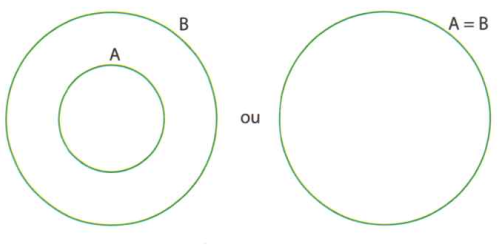
\includegraphics[width=0.7\linewidth]{6FMA03_imagens/imagem1}
	\end{center} 
	Se $A \not\subset B$, há três possibilidades de representação: \\
	\begin{center}
		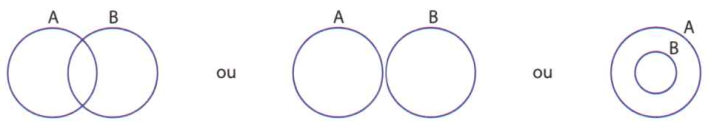
\includegraphics[width=1\linewidth]{6FMA03_imagens/imagem2}
	\end{center} 
	\noindent\textsubscript{-----------------------------------------------------------------------------------------------------------------------------------------------------------}
	\begin{multicols}{2}
		\begin{enumerate}
			\item Em cada item escreva se $A \subset B$ ou se $A \not\subset B$ e desenhe um diagrama.
			\begin{enumerate}[a)]
				\item $A = \{1, 2\} ~~~~~~~~~~ B = \{1, 2, 3\}$ \\\\\\\\\\\\
				\item $A = \{\varnothing, 1, \{2\}\} \\ B = \{\varnothing, \{1\}, 2\}$ \\\\\\\\\\\\\\\\\\
				\item $A = \{1, 2\} ~~~~~~~~~~ B = \{1, 2\}$ \\\\\\\\\\\\
				\item $A = \{1, \{1\}, 2, \{2\}\} \\ B = \{1, \{1\}, 2\}$ \\\\\\\\\\\\
				\item $A = \{1, 2, 3\} \\ B = \{\{1\}, \{2\}, \{3\}\}$ \\\\\\\\\\\\
			\end{enumerate}
			\item Seja $A = \{1, 2, 3\}$. Assinale \textbf{V} (verdadeiro) ou \textbf{F} (falso).
			\begin{enumerate}[a)]
				\item (~~) $1 \in A$ \\\\\\\\\\\\
				\item (~~) $\{1\} \in A$ \\\\\\\\\\\\
				\item (~~) $A \ni 2$ \\\\\\\\\\\\
				\item (~~) $3 \not\in A$ \\\\\\\\\\\\
				\item (~~) $\{1\} \subset A$ \\\\\\\\\\\\
				\item (~~) $\{3\} \subset A$ \\\\\\\\\\\\
				\item (~~) $\{1, 2\} \subset A$ \\\\\\\\\\\\
				\item (~~) $\{1, 2, 3\} \subset A$ \\\\\\\\
				\item (~~) $\{1, 2, 3, 4\} \subset A$ \\\\\\\\\\\\
				\item (~~) $\varnothing \in A$ \\\\\\\\\\\\
				\item (~~) $\varnothing \subset A$ \\\\\\\\\\\\
				\item (~~) $\{1\} \in A$ \\\\\\\\\\\\
				\item (~~) $\{\{1\}\} \subset A$ \\\\\\\\\\\\
				\item (~~) $A \supset \{2, 3\}$ \\\\\\\\
				\item (~~) $A \supset \{\{1\}, 2\}$ \\\\\\\\\\\\
			\end{enumerate}
			\item Assinale \textbf{V} (verdadeiro) ou \textbf{F} (falso).
			\begin{enumerate}[a)]
				\item (~~) $\{1, 2\} \supset \{1\}$ \\\\\\\\\\\\
				\item (~~) $1 \not\in \{2, 3\}$ \\\\\\\\\\\\
				\item (~~) $\{2\} \not\supset \{2, 3\}$ \\\\\\\\\\\\
				\item (~~) $\{1, 2, 3\} \ni 2$ \\\\\\\\\\\\\\
				\item (~~) $\{1, 2, 3\} \not\in 1$ \\\\\\\\\\\\
				\item (~~) $\{1, 1 + 1, 1 + 1 + 1\} \subset \{1, 2, 3\}$ \\\\\\\\\\\\
				\item (~~) $\varnothing \in \varnothing$ \\\\\\\\\\\\
				\item (~~) $\varnothing \in \{\varnothing\}$ \\\\\\\\\\\\
				\item (~~) $\varnothing \subset \varnothing$ \\\\\\\\\\\\
				\item (~~) $\varnothing \in \{1, 2\}$ \\\\\\
				\item (~~) $\varnothing \subset \{1, 2\}$ \\\\\\\\\\\\
				\item (~~) $\{1, 2\} \supset \{1, 2\}$ \\\\\\\\\\\\
				\item (~~) $3 = \{3\}$ \\\\\\\\\\\\
				\item (~~) $\{1\} \supset \{1, 2\}$ \\\\\\\\\\\\
				\item (~~) $2 \in 2$ \\\\\\\\\\\\
				\item (~~) $\{\varnothing\} \subset \varnothing$ \\\\\\\\
				\item (~~) $\{1\} \in \{0, \{1\}, 2\}$ \\\\\\\\\\\\
			\end{enumerate}
			% 7 a 9
			\item Em cada item escreva se $A \subset B$ ou se $A \not\subset B$ e desenhe um diagrama.
			\begin{enumerate}[a)]
				\item $A = \{1, 2, 3\}$ e $B = \{2, 3, 4, 5\}$. \\\\\\\\\\\\\\\\\\\\\\\\\\\\
				\item $A = \{1, \{1\}, 2\}$ e $B = \{1, \{1\}, 2, \{2\}\}$. \\\\\\\\\\\\\\\\\\\\\\
				\item $A = \{5, 6\}$ e $B = \{1, 3, 5, \{6\}\}$. \\\\\\\\\\\\\\\\\\\\\\\\\\\\
				\item $A = \{3, \{3\}, 5, \{7\}\}$ e $B = \{3, \{3\}, 5, \{5\}, 7, \{7\}\}$. \\\\\\\\\\\\\\\\\\\\\\\\\\\\
				\item $A = \{5, 6, 7, 8\}$ e $B = \{5, 6\}$.
			\end{enumerate}
			\item Considere as afirmações abaixo e assinale a alternativa correta.
			\begin{enumerate}[I.]
				\item $1 \subset \{1, 2, 3\}$
				\item $\{3\} \in \{0, 1, 2, 3\}$
				\item $\{8, 7\} \subset \{7, 8\}$
				\item $5 \in \{3, 4, 5\}$
			\end{enumerate}
			\begin{enumerate}[a)]
				\item Somente I e IV são verdadeiras.
				\item Somente II e III são verdadeiras.
				\item Somente III e IV são verdadeiras.
				\item Somente I é verdadeira.
				\item Todas são verdadeiras. 
			\end{enumerate}
			\item Se $A = \{\varnothing, 5, \{5\}, \{5, 6\}\}$, então:
			\begin{enumerate}[a)]
				\item $\{5, 6\} \subset A$
				\item $\{5\} \in A$
				\item $\varnothing \not\in A$
				\item $6 \in A$
				\item $5 \subset A$
			\end{enumerate}
		\end{enumerate}
		$~$ \\ $~$ \\ $~$ \\ $~$ \\ $~$ \\ $~$ \\ $~$ \\ $~$ \\ $~$ \\ $~$ \\ $~$ \\ $~$ \\ $~$ \\ $~$ \\ $~$ \\ $~$ \\ $~$ \\ $~$ \\ $~$ \\ $~$ \\ $~$ \\ $~$ \\ $~$ \\ $~$ \\ $~$ \\ $~$ \\ $~$ \\ $~$ \\ $~$ \\ $~$ \\ $~$ \\ $~$ \\ $~$ \\ $~$ \\ $~$ \\ $~$ \\ $~$ \\ $~$ \\ $~$ \\ $~$ \\ $~$ \\ $~$ \\ $~$ \\ $~$ \\ $~$ \\ $~$ \\ $~$ \\ $~$ \\ $~$ \\ $~$ \\ $~$ \\ $~$ \\ $~$ \\ $~$ \\ $~$ \\ $~$ \\ $~$ \\ $~$ \\ $~$ \\ $~$ \\ $~$ \\ $~$ \\ $~$ \\
	\end{multicols}
\end{document}